\documentclass[twoside]{book}

% Packages required by doxygen
\usepackage{fixltx2e}
\usepackage{calc}
\usepackage{doxygen}
\usepackage[export]{adjustbox} % also loads graphicx
\usepackage{graphicx}
\usepackage[utf8]{inputenc}
\usepackage{makeidx}
\usepackage{multicol}
\usepackage{multirow}
\PassOptionsToPackage{warn}{textcomp}
\usepackage{textcomp}
\usepackage[nointegrals]{wasysym}
\usepackage[table]{xcolor}

% Font selection
\usepackage[T1]{fontenc}
\usepackage[scaled=.90]{helvet}
\usepackage{courier}
\usepackage{amssymb}
\usepackage{sectsty}
\renewcommand{\familydefault}{\sfdefault}
\allsectionsfont{%
  \fontseries{bc}\selectfont%
  \color{darkgray}%
}
\renewcommand{\DoxyLabelFont}{%
  \fontseries{bc}\selectfont%
  \color{darkgray}%
}
\newcommand{\+}{\discretionary{\mbox{\scriptsize$\hookleftarrow$}}{}{}}

% Page & text layout
\usepackage{geometry}
\geometry{%
  a4paper,%
  top=2.5cm,%
  bottom=2.5cm,%
  left=2.5cm,%
  right=2.5cm%
}
\tolerance=750
\hfuzz=15pt
\hbadness=750
\setlength{\emergencystretch}{15pt}
\setlength{\parindent}{0cm}
\setlength{\parskip}{0.2cm}
\makeatletter
\renewcommand{\paragraph}{%
  \@startsection{paragraph}{4}{0ex}{-1.0ex}{1.0ex}{%
    \normalfont\normalsize\bfseries\SS@parafont%
  }%
}
\renewcommand{\subparagraph}{%
  \@startsection{subparagraph}{5}{0ex}{-1.0ex}{1.0ex}{%
    \normalfont\normalsize\bfseries\SS@subparafont%
  }%
}
\makeatother

% Headers & footers
\usepackage{fancyhdr}
\pagestyle{fancyplain}
\fancyhead[LE]{\fancyplain{}{\bfseries\thepage}}
\fancyhead[CE]{\fancyplain{}{}}
\fancyhead[RE]{\fancyplain{}{\bfseries\leftmark}}
\fancyhead[LO]{\fancyplain{}{\bfseries\rightmark}}
\fancyhead[CO]{\fancyplain{}{}}
\fancyhead[RO]{\fancyplain{}{\bfseries\thepage}}
\fancyfoot[LE]{\fancyplain{}{}}
\fancyfoot[CE]{\fancyplain{}{}}
\fancyfoot[RE]{\fancyplain{}{\bfseries\scriptsize Generated on Sun Sep 6 2015 18\+:39\+:36 for My Project by Doxygen }}
\fancyfoot[LO]{\fancyplain{}{\bfseries\scriptsize Generated on Sun Sep 6 2015 18\+:39\+:36 for My Project by Doxygen }}
\fancyfoot[CO]{\fancyplain{}{}}
\fancyfoot[RO]{\fancyplain{}{}}
\renewcommand{\footrulewidth}{0.4pt}
\renewcommand{\chaptermark}[1]{%
  \markboth{#1}{}%
}
\renewcommand{\sectionmark}[1]{%
  \markright{\thesection\ #1}%
}

% Indices & bibliography
\usepackage{natbib}
\usepackage[titles]{tocloft}
\setcounter{tocdepth}{3}
\setcounter{secnumdepth}{5}
\makeindex

% Hyperlinks (required, but should be loaded last)
\usepackage{ifpdf}
\ifpdf
  \usepackage[pdftex,pagebackref=true]{hyperref}
\else
  \usepackage[ps2pdf,pagebackref=true]{hyperref}
\fi
\hypersetup{%
  colorlinks=true,%
  linkcolor=blue,%
  citecolor=blue,%
  unicode%
}

% Custom commands
\newcommand{\clearemptydoublepage}{%
  \newpage{\pagestyle{empty}\cleardoublepage}%
}


%===== C O N T E N T S =====

\begin{document}

% Titlepage & ToC
\hypersetup{pageanchor=false,
             bookmarks=true,
             bookmarksnumbered=true,
             pdfencoding=unicode
            }
\pagenumbering{roman}
\begin{titlepage}
\vspace*{7cm}
\begin{center}%
{\Large My Project \\[1ex]\large 1.\+0 }\\
\vspace*{1cm}
{\large Generated by Doxygen 1.8.10}\\
\vspace*{0.5cm}
{\small Sun Sep 6 2015 18:39:36}\\
\end{center}
\end{titlepage}
\clearemptydoublepage
\tableofcontents
\clearemptydoublepage
\pagenumbering{arabic}
\hypersetup{pageanchor=true}

%--- Begin generated contents ---
\chapter{Hierarchical Index}
\section{Class Hierarchy}
This inheritance list is sorted roughly, but not completely, alphabetically\+:\begin{DoxyCompactList}
\item \contentsline{section}{Client}{\pageref{class_client}}{}
\item \contentsline{section}{Constant}{\pageref{class_constant}}{}
\item \contentsline{section}{Server}{\pageref{class_server}}{}
\item Thread\begin{DoxyCompactList}
\item \contentsline{section}{W\+Thread}{\pageref{class_w_thread}}{}
\end{DoxyCompactList}
\item Unicast\+Remote\+Object\begin{DoxyCompactList}
\item \contentsline{section}{Matrix}{\pageref{class_matrix}}{}
\end{DoxyCompactList}
\item Remote\begin{DoxyCompactList}
\item \contentsline{section}{Matrix\+\_\+mnoz}{\pageref{interface_matrix__mnoz}}{}
\begin{DoxyCompactList}
\item \contentsline{section}{Matrix}{\pageref{class_matrix}}{}
\end{DoxyCompactList}
\end{DoxyCompactList}
\end{DoxyCompactList}

\chapter{Class Index}
\section{Class List}
Here are the classes, structs, unions and interfaces with brief descriptions\+:\begin{DoxyCompactList}
\item\contentsline{section}{\hyperlink{class_client}{Client} }{\pageref{class_client}}{}
\item\contentsline{section}{\hyperlink{class_constant}{Constant} }{\pageref{class_constant}}{}
\item\contentsline{section}{\hyperlink{class_matrix}{Matrix} }{\pageref{class_matrix}}{}
\item\contentsline{section}{\hyperlink{interface_matrix__mnoz}{Matrix\+\_\+mnoz} }{\pageref{interface_matrix__mnoz}}{}
\item\contentsline{section}{\hyperlink{class_server}{Server} }{\pageref{class_server}}{}
\item\contentsline{section}{\hyperlink{class_w_thread}{W\+Thread} }{\pageref{class_w_thread}}{}
\end{DoxyCompactList}

\chapter{Class Documentation}
\hypertarget{class_client}{}\section{Client Class Reference}
\label{class_client}\index{Client@{Client}}
\subsection*{Static Public Member Functions}
\begin{DoxyCompactItemize}
\item 
\hypertarget{class_client_ac4219c51358857184ceeb023ada3d8ae}{}static void {\bfseries main} (String args\mbox{[}$\,$\mbox{]})  throws Remote\+Exception, 			\+Not\+Bound\+Exception \label{class_client_ac4219c51358857184ceeb023ada3d8ae}

\end{DoxyCompactItemize}


The documentation for this class was generated from the following file\+:\begin{DoxyCompactItemize}
\item 
D\+:/java 2/work\+\_\+srir/\+Matrix/\+Doxygen\+\_\+src/Client.\+java\end{DoxyCompactItemize}

\hypertarget{class_constant}{}\section{Constant Class Reference}
\label{class_constant}\index{Constant@{Constant}}
\subsection*{Static Public Attributes}
\begin{DoxyCompactItemize}
\item 
\hypertarget{class_constant_abbee07791e6042920828ed533efabbb7}{}static final String {\bfseries R\+M\+I\+\_\+\+I\+D} = \char`\"{}Matrix\char`\"{}\label{class_constant_abbee07791e6042920828ed533efabbb7}

\item 
\hypertarget{class_constant_a3724cc2248533bef4665190d2acb5fbb}{}static final int {\bfseries R\+M\+I\+\_\+\+P\+O\+R\+T} = 8082\label{class_constant_a3724cc2248533bef4665190d2acb5fbb}

\end{DoxyCompactItemize}


The documentation for this class was generated from the following file\+:\begin{DoxyCompactItemize}
\item 
D\+:/java 2/work\+\_\+srir/\+Matrix/\+Doxygen\+\_\+src/Constant.\+java\end{DoxyCompactItemize}

\hypertarget{class_matrix}{}\section{Matrix Class Reference}
\label{class_matrix}\index{Matrix@{Matrix}}
Inheritance diagram for Matrix\+:\begin{figure}[H]
\begin{center}
\leavevmode
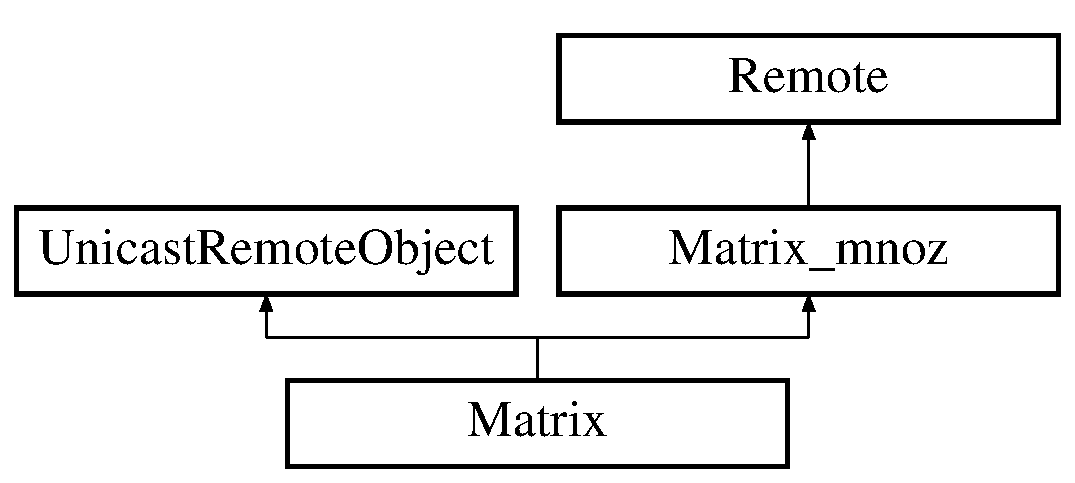
\includegraphics[height=3.000000cm]{class_matrix}
\end{center}
\end{figure}
\subsection*{Public Member Functions}
\begin{DoxyCompactItemize}
\item 
\hypertarget{class_matrix_a20d3fe31c44ec0cb91bdbd5f093cf9aa}{}boolean {\bfseries licz} (int n, double\mbox{[}$\,$\mbox{]}\mbox{[}$\,$\mbox{]} A)\label{class_matrix_a20d3fe31c44ec0cb91bdbd5f093cf9aa}

\item 
\hypertarget{class_matrix_a6bdc81171a0fa46d12295cd70e3eb0f5}{}boolean {\bfseries oblicz} (int k, int n, double\mbox{[}$\,$\mbox{]}\mbox{[}$\,$\mbox{]} A, double\mbox{[}$\,$\mbox{]}\mbox{[}$\,$\mbox{]} X)\label{class_matrix_a6bdc81171a0fa46d12295cd70e3eb0f5}

\item 
\hypertarget{class_matrix_a603f88c2a9748145f46ae1bf4320f135}{}double\mbox{[}$\,$\mbox{]}\mbox{[}$\,$\mbox{]} {\bfseries transpozycja} (double A\mbox{[}$\,$\mbox{]}\mbox{[}$\,$\mbox{]}, int n)  throws Remote\+Exception \label{class_matrix_a603f88c2a9748145f46ae1bf4320f135}

\end{DoxyCompactItemize}


The documentation for this class was generated from the following file\+:\begin{DoxyCompactItemize}
\item 
D\+:/java 2/work\+\_\+srir/\+Matrix/\+Doxygen\+\_\+src/Matrix.\+java\end{DoxyCompactItemize}

\hypertarget{interface_matrix__mnoz}{}\section{Matrix\+\_\+mnoz Interface Reference}
\label{interface_matrix__mnoz}\index{Matrix\+\_\+mnoz@{Matrix\+\_\+mnoz}}
Inheritance diagram for Matrix\+\_\+mnoz\+:\begin{figure}[H]
\begin{center}
\leavevmode
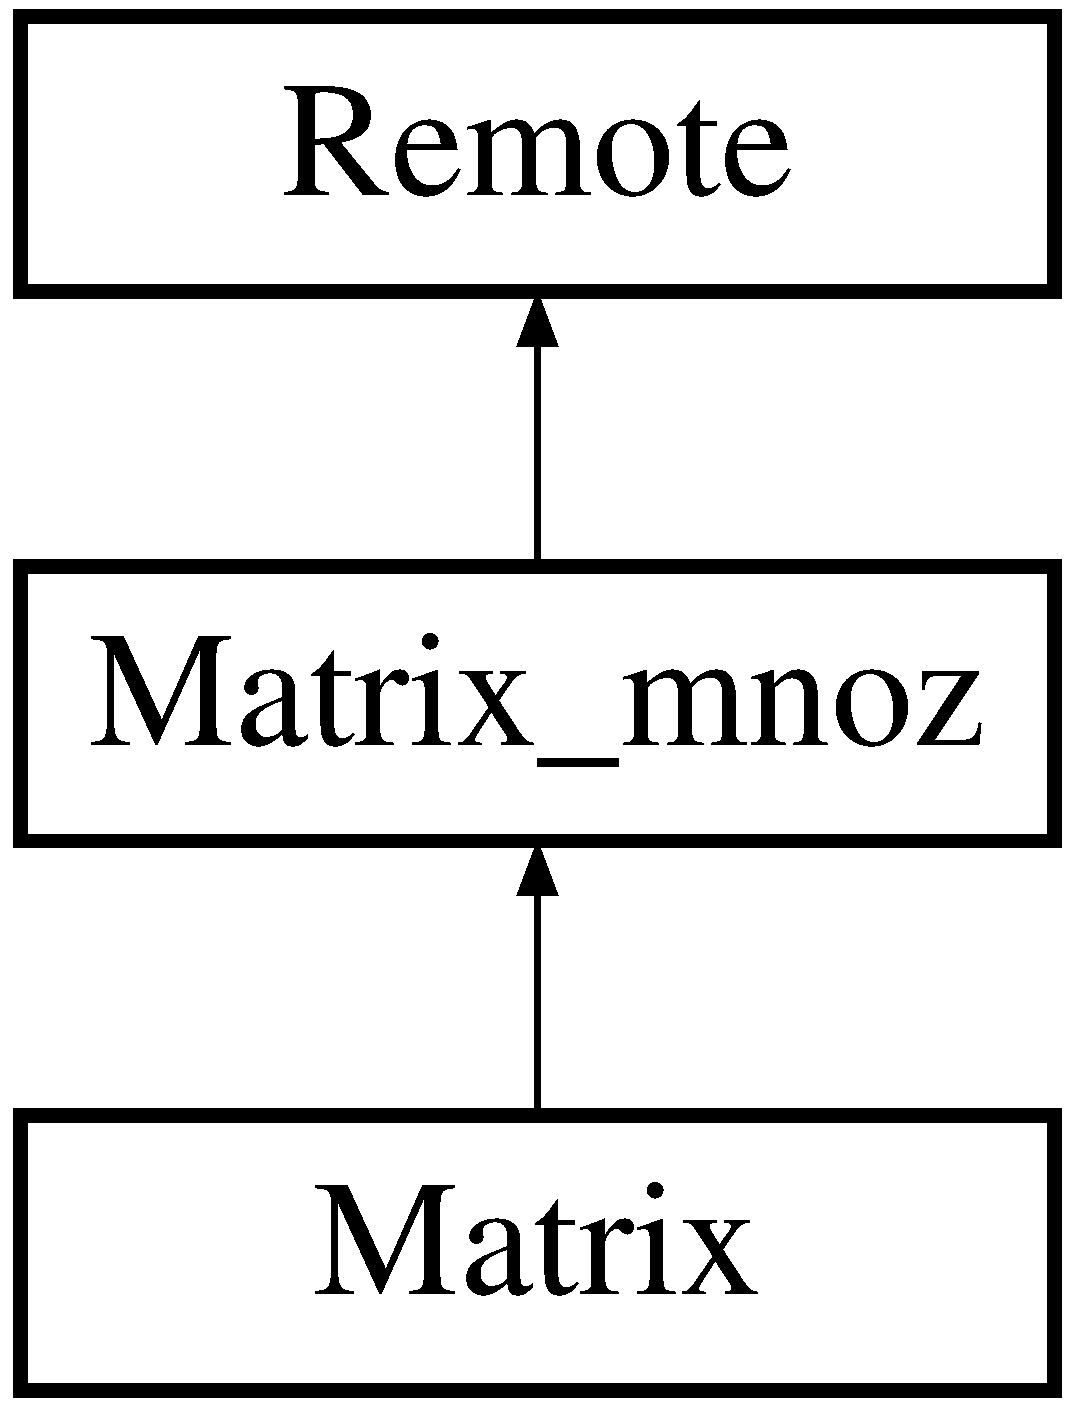
\includegraphics[height=3.000000cm]{interface_matrix__mnoz}
\end{center}
\end{figure}
\subsection*{Public Member Functions}
\begin{DoxyCompactItemize}
\item 
\hypertarget{interface_matrix__mnoz_a6dc3f28e37b1de67d11370eabc219ecd}{}double\mbox{[}$\,$\mbox{]}\mbox{[}$\,$\mbox{]} {\bfseries transpozycja} (double a\mbox{[}$\,$\mbox{]}\mbox{[}$\,$\mbox{]}, int m)  throws Remote\+Exception\label{interface_matrix__mnoz_a6dc3f28e37b1de67d11370eabc219ecd}

\end{DoxyCompactItemize}


The documentation for this interface was generated from the following file\+:\begin{DoxyCompactItemize}
\item 
D\+:/java 2/work\+\_\+srir/\+Matrix/\+Doxygen\+\_\+src/Matrix\+\_\+mnoz.\+java\end{DoxyCompactItemize}

\hypertarget{class_server}{}\section{Server Class Reference}
\label{class_server}\index{Server@{Server}}
\subsection*{Static Public Member Functions}
\begin{DoxyCompactItemize}
\item 
\hypertarget{class_server_ad90c92078da8d9c8a084e7cbc6cff4af}{}static void {\bfseries main} (String args\mbox{[}$\,$\mbox{]})\label{class_server_ad90c92078da8d9c8a084e7cbc6cff4af}

\end{DoxyCompactItemize}


The documentation for this class was generated from the following file\+:\begin{DoxyCompactItemize}
\item 
D\+:/java 2/work\+\_\+srir/\+Matrix/\+Doxygen\+\_\+src/Server.\+java\end{DoxyCompactItemize}

\hypertarget{class_w_thread}{}\section{W\+Thread Class Reference}
\label{class_w_thread}\index{W\+Thread@{W\+Thread}}
Inheritance diagram for W\+Thread\+:\begin{figure}[H]
\begin{center}
\leavevmode
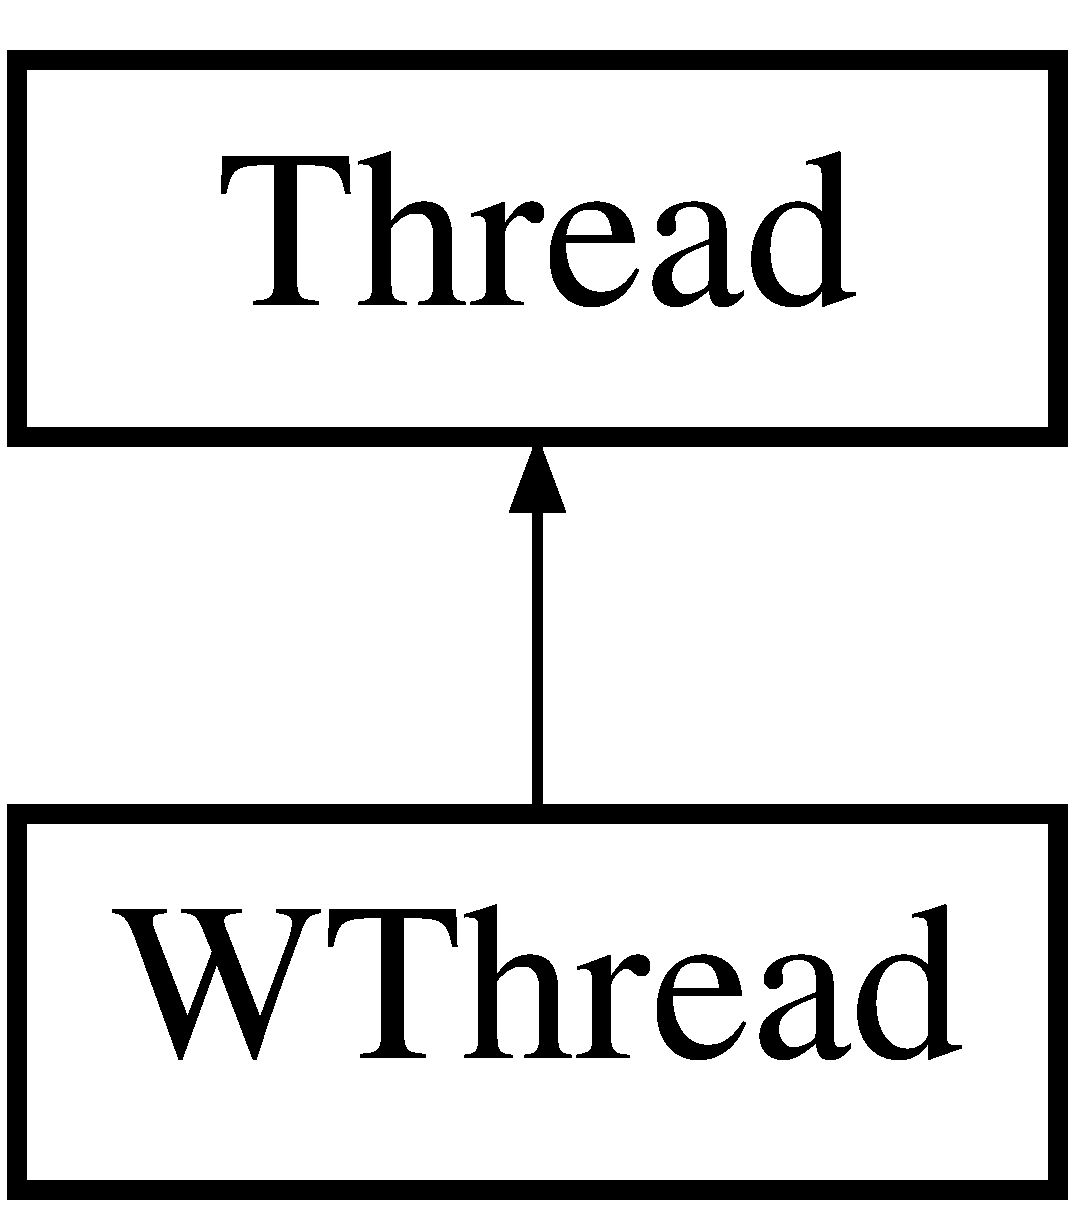
\includegraphics[height=2.000000cm]{class_w_thread}
\end{center}
\end{figure}
\subsection*{Public Member Functions}
\begin{DoxyCompactItemize}
\item 
\hypertarget{class_w_thread_afec76e07756953171b637b156f481830}{}{\bfseries W\+Thread} (int start, int end, int n, double\mbox{[}$\,$\mbox{]}\mbox{[}$\,$\mbox{]} A)\label{class_w_thread_afec76e07756953171b637b156f481830}

\item 
\hypertarget{class_w_thread_a961e88e950dcd5388bd47bb94a738127}{}void {\bfseries run} ()\label{class_w_thread_a961e88e950dcd5388bd47bb94a738127}

\end{DoxyCompactItemize}


The documentation for this class was generated from the following file\+:\begin{DoxyCompactItemize}
\item 
D\+:/java 2/work\+\_\+srir/\+Matrix/\+Doxygen\+\_\+src/W\+Thread.\+java\end{DoxyCompactItemize}

%--- End generated contents ---

% Index
\backmatter
\newpage
\phantomsection
\clearemptydoublepage
\addcontentsline{toc}{chapter}{Index}
\printindex

\end{document}
